\documentclass[border=1mm]{standalone}

\usepackage{tikz}
\usetikzlibrary{arrows,shapes.gates.logic.US,shapes.gates.logic.IEC,calc}
\begin{document}
\thispagestyle{empty}
\tikzstyle{branch}=[fill,shape=circle,minimum size=3pt,inner sep=0pt]
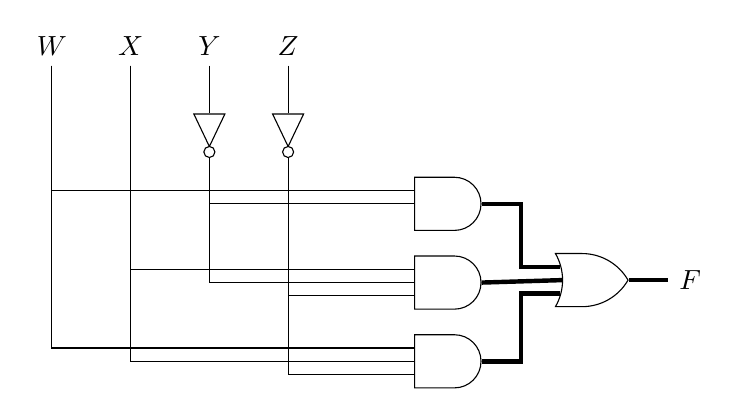
\begin{tikzpicture}[label distance=2mm]

\node (w) at (0,0) {$W$};
\node (x) at (1,0) {$X$};
\node (y) at (2,0) {$Y$};
\node (z) at (3,0) {$Z$};

\node[not gate US, draw, rotate=-90] at ($(y)+(0,-1)$) (Not2) {};
\node[not gate US, draw, rotate=-90] at ($(z)+(0,-1)$) (Not1) {};
\node[and gate US, draw, logic gate inputs=nnn, font=\bfseries\color{red}] at ($(y)+(3,-2)$) (and1) {};
\node[and gate US, draw, logic gate inputs=nnn, font=\bfseries\color{red}] at ($(and1)+(0,-1)$) (and2) {};
\node[and gate US, draw, logic gate inputs=nnn, font=\bfseries\color{red}] at ($(and2)+(0,-1)$) (and3) {};
\node[or gate US, draw, logic gate inputs=nnn, anchor=input 1] at ($(and1.output -| and2.output -| and3.output)+(1,-.8)$) (or) {};

\draw (w) |- (and1.input 1);
\draw (w) |- (and3.input 1);

\draw (x) |- (and2.input 1);
\draw (x) |- (and3.input 2);

\draw (y) |- (Not2.input);
\draw (z) |- (Not1.input);

\draw (Not2.output) |- (and1.input 2);
\draw (Not2.output) |- (and2.input 2);

\draw (Not1.output) |- (and2.input 3);
\draw (Not1.output) |- (and3.input 3);


\draw [ ultra thick] (and1.output) -- ++(0.5cm,0) |- (or.input 1) 
        node [shift={(-0.65em,0.75ex)}, font=\tiny] {};
\draw [ ultra thick] (and2.output) -- (or.input 2) 
        node [shift={(0.65em,0ex)}, , font=\tiny] {};
\draw [ ultra thick] (and3.output) -- ++(0.5cm,0) |- (or.input 3) 
        node [shift={(-0.66em,-0.75ex)}, , font=\tiny] {};

\draw [, ultra thick] (or.east) -- ++(0.5cm,0) node [right] {$F$};


\end{tikzpicture}
\end{document} 
